%******************************FORMATIERUNG****************************************
\documentclass[a4paper, 12pt]{article}
\usepackage{scrpage2}
\usepackage{todonotes}
\usepackage{amssymb}
\usepackage{amsmath}
\usepackage{esvect}
\usepackage{caption}
\pagestyle{scrheadings}
\clearscrheadfoot
\setheadsepline{.5pt}
\setfootsepline{.5pt}
\automark[section]{chapter}
\ihead{\headmark}
\ohead{\pagemark}
\usepackage[ngerman]{babel}
\usepackage[utf8]{inputenc}
\usepackage{graphicx}
\usepackage[space]{grffile}
\usepackage{setspace}
\usepackage[T1]{fontenc}
\usepackage[section]{placeins}
\usepackage{listings}
\renewcommand{\lstlistingname}{Quellcode-Auszug}	
\definecolor{lsgreen}{rgb}{0,.5,0}
\definecolor{lsred}{rgb}{.7,0,0}
\definecolor{lsorange}{rgb}{.9,.5,0}
\definecolor{lsgray}{rgb}{.5,.5,.5}
\lstloadlanguages{[Sharp]C}
\lstset{
	frame=tb,
	aboveskip=10mm,
	belowskip=5mm,
	showstringspaces=false,
	columns=flexible,
	captionpos=b,
	basicstyle={\scriptsize\ttfamily},
	numbers=left,
	numberstyle=\tiny\color{lsgray},
	keywordstyle=\color{blue},
	commentstyle=\color{lsorange},
	stringstyle=\color{lsgreen},
	breaklines=true,
	breakatwhitespace=true,
	rulecolor=\color{lsgray},
	xleftmargin=7mm,
	tabsize=3
}
\newcommand{\changefont}[3]{
\fontfamily{#1} \fontseries{#2} \fontshape{#3} \selectfont}
\usepackage{datetime}
\newdateformat{monthyeardate}{%
  \monthname[\THEMONTH] \THEYEAR}
\usepackage{geometry}
\geometry{verbose,a4paper,tmargin=30mm,bmargin=30mm,lmargin=35mm,rmargin=25mm}
\usepackage[numbers,square]{natbib}
\usepackage[
	breaklinks=true,
	pdfauthor={Laura Anger, Vera Brockmeyer, Britta Boerner, Anna Bolder},
	pdftitle={Interaction Lab},
	pdftoolbar=true,
	%pdfsubject={},
	colorlinks=true,
	linkcolor=blue,
	citecolor=blue,
	urlcolor=blue,
	linktocpage=true
	]{hyperref}
\usepackage{algorithmicx}
\usepackage{multicol}
\usepackage{multirow}
\usepackage[ruled]{algorithm}
\usepackage{algpseudocode}
\usepackage{pdfpages}
\usepackage[
	font=small,
	labelfont=bf, 
	format=plain,
	indention=1cm
	]{caption}
\setlength{\parindent}{0pt} 
\setlength{\parskip}{.5em}
\usepackage{color}
\definecolor{myColor}{rgb}{0.8,0.8,0.8}
\newcommand{\Absatzbox}[1]{\parbox[0pt][2em][c]{0cm}{}}
\usepackage{listings}
\usepackage{tabularx}

%*****************************ENDE FORMATIERUNG****************************************

\begin{document}
%\linespread{1.2}
%\changefont{ppl}{m}{n}

%INHALTSVERZEICHNIS
%\pagenumbering{arabic}
%\input{main/Inhaltsverzeichnis.tex}

\thispagestyle{empty}
\begin{center}
	
\includegraphics[width=5cm]{Images/logo_TH}\\[12ex]
	{\Huge\textbf{Project Documentation}}\\[8ex]
	\rule{.8\textwidth}{.2pt}
	{\Large\\[1ex] \textbf{Interactive Lighting Detector}}\\
	\rule{.8\textwidth}{.2pt}\\[10ex]
	written by\\[2ex]
	\begin{tabular}{ll}
		Vera Brockmeyer &(Matrikelnr. 11077082)\\
		Laura Anger &(Matrikelnr. 11086356)\\ 
	\end{tabular}\\[10ex]
	\textbf{Image Processing in SS 2017}\\			
\end{center}
\vfill
\begin{flushleft}
	{\bf Supervisor:}\\
	Prof. Dr. Dietmar Kunz \\
	Institute for Media- and Phototechnology
\end{flushleft}
\newpage
	\tableofcontents
	\newpage
	%\listoffigures
	%\newpage
	%\listoftables
	%\newpage


\section{Introduction}\label{sec:Introduction}
The detection of digital image forgery is an actual research topic, which analyses various image properties to get a conclusion about the authenticity of a digital image. It can be divided into two sections~\cite{4284575}. The first section is the source digital camera identification. It considers image properties like lens aberrations, sensor imperfections or use a colour filter array (CFA) interpolation to analyse the suspicious items. Those mentioned properties can give an assumption on the camera or even the camera model, which was used to capture the picture.

The other section is the actual image forgery analysis. A common method to detect the application or device that was used to save the image file is the analysis of JPEG patterns. Each has an individual JPEG pattern which can be extracted and compared to a database of acknowledged patterns. Another approach for image forgery analysis is the detailed observation of the chromatic aberration camera response function (CRF) that can give conclusions about manipulations in form of retouching or composing of new image content. 

Due to the assumption that different images are taken under different light conditions, the manipulative composition of two images can be often detected by analysing the light vectors of various objects depicted in the image. But this method is also very difficult because it needs an image sequence of the scene to estimate the 3-dimensional light direction successfully with established algorithms. This is not very useful in reality because in most cases only the suspect image is available without any information about its real environment. Nevertheless, there exists an approach by Johnston and Farid~\cite{Johnson} that can rather estimate the object's light direction under some pre defined assumptions even from single images with a common least square approach. The assumptions are clearly defined and result in a simplified light model that is related to an infinite light source and a constant reflection values of the object's surface.

\subsection{Motivation}\label{sec:Motivation}
In the last decade, it became more easily to create an image forgery for everyone. Software applications like \textit{Adobe Photoshop} or \textit{Gimp} and almost every mobile phone or social media platform offers possibilities to sophisticate digital images. Every user can manipulate images or compose a new image of various other images without any significant knowledge. For example, two portraits of prominent people can be combined in a way that the impression of a relationship accrues which does not really exist. If this is made in an imperfect way the forgeries can be recognised very quickly by the human visual system but if they are made in a professional way it is quite challenging to detect the manipulation. 

In this case, a professional analysis tool is required to give a reliable rating which can stand in court as evidence. As mentioned, a main problem of the analysis is that many approaches ask for a sequence of images from the scene for trustworthy and validated results but in most cases only the suspect image is available. Thus, an approach which estimates the light vector under some refused assumption has to be used and eventually confirmed by other image forgery detection methods. 

\subsection{Project Goal}\label{sec:Project Goal}
According to the previous sections, the project goal is to implement and evaluate the approach of Johnston~\cite{Johnson} in \textit{C++} with an adequate \textit{Qt} Graphic User Interface (GUI). This GUI offers a segmentation of the object of interest, as well as an interactive selection of the most suitable contour part, to estimate the light direction. The latter is an important requirement of the Johnston approach. To validate the results, several test images have to be captured with a simulated infinite light source. The infinite light source can be the sun on a cloudless day, for example. A sun clock needs to be added to the test scene to verify the current light direction and various objects with a simple and even shape complete it. All resulting vectors and contours are printed in the actual image or respectively saved in a text file for the following evaluation.



\newpage



















\section{State of the Art} \label{sec:StateOfTheArt}
\todo[inline, color=yellow]{Laura}
In the following sections the basic scientific knowledge to understand the \textit{Lighting Detector}, whose functionality is explained in section~\ref{sec:System}, is presented.\\
A general introduction to image forensic is given in section~\ref{sec:imageForensic}.
Furthermore, other approaches using light vectors to detect image manipulation are shortly presented in section~\ref{sec:otherApproaches}.


\subsection{Image Forensic}\label{sec:imageForensic}
\todo[inline, color=yellow]{Laura}
In \cite{4284575} the authors claim image forensic to become more important over the years. Furthermore, they divide the field in two approaches. First of all image forensic can be used to identify the recording device of an image. This can, inter alia, be done by taking sensor imperfections, like for example pixel defects, or the lens aberration of the camera into consideration. \\
The second field of interest is the detection of image forgery \cite{4806202}. Besides of using the camera response function there can be other details in the image which can be informative whether an image is real or a forgery. For example the light situation in an image must be consistent. This can be proofed by calculating light vectors in various points in the image. The \textit{Light Detector} is using exactly this method (compare section~\ref{sec:System}). Related approaches are described briefly in section~\ref{sec:otherApproaches}.


\subsection{Related Approaches} \label{sec:otherApproaches}
\todo[inline, color=yellow]{Laura}
The \textit{Lighting Detector} was implemented according to the paper by Johnson and Farid \cite{Johnson}. The foundation of their assumptions where set in 2001 by the publication of Nillius and Eklundh on an "\textit{automatic estimation of the projected light source direction}" \cite{990650}. Where as the earlier theory is taking three dimensional surface normals to determine the light vectors pointing into the direction if the light source, the newer approach by Johnson and Farid uses only one image, and therefore two dimensional surface normals, to achieve the same goal. \\
An other related approach, which is also presented by Johnson and Farid estimates the three dimensional light direction from the light's reflections in the eyes of human. Therefore they determine the light vector by using the surface normal and the view direction of the person \cite{johnson06specular}.

\textcolor{red}{Hast du noch andere Ansätze gefunden die enen ähnlichen Ansatz verfolgen??? Alle paper die ich sonst gefunden habe, fahren einen anderen Ansatz. HAHA, warum nur?} 


\newpage

\section{Materials}\label{sec:Materials}
\todo[inline, color=red]{Laura}

\subsection{Hardware}\label{sec:Hardware}
\todo[inline, color=red]{Laura}


%\subsubsection{Computer}\label{sec:Computer}
%\todo[inline, color=red]{Laura}
%\textcolor{red}{@??: Vielleicht möchtest du die Tabelle einfach übernehmen und nur die Daten des PCs ändern?}\\

\begin{table}
	\centering
	\begin{tabular}{|l|l|}
		\hline
		\Absatzbox{}
		\textbf{CGPC6}& \textbf{Beschreibung} \\
		\hline
		Prozessor & Intel Core i7 6700 CPU @ $4\times3.4-4.0\,$GHz \\
		\hline
		Arbeitsspeicher & $16\,$GB \\
 		\hline 
		Grafikkarte & NVIDIA GeForce GTX 980\\
		\hline
		Betriebssystem & Windows 10 Education 64 bit \\
		\hline
		Schnittstellen & $2\times$ USB 3.0, $5\times$ USB 2.0, $1\times $ HDMI\\
		\hline
	\end{tabular}
	\caption[Übersicht technische Daten des Computers für \emph{Unity}-Simulation]{Übersicht der technischen Daten des Computers für die \emph{Unity}-Simulation.}
	\label{tab:Computer}
\end{table}




\subsection{Software}
\todo[inline, color=red]{Laura}



\newpage

\section{System}\label{sec:System}
\todo[inline, color=red]{???}



\newpage
\section{Evaluation} \label{sec:Evaluation}
\todo[inline, color=red]{Vera und Laura: Stichpunkte}
\todo[inline, color=red]{Vera: Ausformulierung}

Stichpunkte Laura:\\
Allgemein:\\
\begin{itemize}
\item es ist auffällig, dass die autoren bei den Komplexeren Aufnahmen (mit den Promis) keine einzelne Lichtvekoren mehr einzeichnen. 
\item Es wurde versucht möglichst homogene Objekte zum testen zu nehmen (vor allem der zweite Satz der Testbilder)
\end{itemize}

Beobachtungen unserer Versuche:\\
\begin{itemize}
\item lediglich eine visuelle Auswertung
\item Wir bekomen immer wieder Vektoren, die in die richtige Richtung zeigen  (bzw. um 180 gedrehte Vektoren) aber der Algorihtmus funtkioniert nicht zuverlässig
\item Da Ergebnisse eher zufällig wirken, macht es keinen Sinn die drei Ansätze direkt miteinander zu vergleichen, der zweite Ansatz scheint jedoch am häufigste richtig zu liegen.
\end{itemize}





\newpage
\section{Project Management} \label{sec:pm}
\todo[inline, color=yellow]{Laura}
In this section the planning and the management of the \textit{Lighting Lab} is described. As there were only two persons involved this project the following part is going to be a bit more compressed than the reader might expected it.\\
To give the customer an all-encompassing idea about the \textit{Interaction Lab} a project proposal was handed in, which is written in German. It is divided in two sections. First of all a motivation is given and afterwards the exercise, which should be implemented is determined. It is translated into English and can be found in section~{sec:ProjectProposal}. \\ 
Before starting the actual project it is wise to make some mindful project plans in order to organize the project. First of all a catalogue of requirements and specifications (compare section~\ref{sec:PMcatalogue}) was written to formulate all important basic information of the project. \\
The project structure plan, which is presented in section~\ref{sec:StructurePlan}, serves to arrange the work packages of the project in a sorted way. The relating milestone description can found in section~\ref{sec:Milestones}. \\
For staying in time while the implementation phase, a time exposure is required (compare section~\ref{sec:timeExposure}).\\
A list with all early detectable risks can be found in the table in section~\ref{sec:risks}.


\subsection{Project Proposal}\label{sec:ProjectProposal}
\todo[inline, color=yellow]{Laura}

\textbf{Motivation} \\
Due to progressive changes in image processing programs and high-resolution images, the manipulation of digital images is became easier. A common form of manipulation is the so-called "\textit{image splicing}". Therefore image regions of at least two images where combined to a new one. The transitions between the individual image parts can get invisible for the user by using accurate and user-friendly image processing tools.
According to \cite{Hsu2006DetectingIS} there is is still no algorithm, which makes images completely forgery-proof by adding watermarks to it. There is put much effort in the integrity of images and the recognition of manipulated image parts, despite the lack of prior knowledge of the image content. This should be improved by the \textit{Interaction Lab}. An algorithm should be established, which proofs the consistence in light directions on various surfaces presented on an image. The light vectors will be conveniently estimated to give an assertion on whether the image is manipulated or not.\\

\textbf{Work Steps} \\
Until now there is no implementation given by \textit{OpenCV}, which estimates the light vector of an infinite light source on one surface and compares it with the according vector of another surface in the same image. An approach in the programming language \textit{C++} should be implemented using the assumptions of Johnson and Farid \cite{Johnson} to compute, analyse and visualize the light vectors. \\The following work stages are necessary: 

\begin{itemize}
\item Creation of test images with an infinite light source, e.g. in nature on a sunny day 
\item Implementation of a GUI for visualize the approach
\item Implementation of the algorithm of Johnson and Farid \cite{Johnson}
\item Optional: The approach might be amended by also taking a local (not infinite) light source into consideration \cite{Johnson}
\end{itemize}


\subsection{Catalogue of Requirements and Specification} \label{sec:PMcatalogue}
\todo[inline, color=yellow]{Laura}
Project Manager: Laura Anger \\
Team Member: Vera Brockmeyer \\
Supervisor: Prof. Dr. Dietmar Kunz\\ \\
\textbf{Project Goals}\\ \\
This project aims to implement an interactive image forensic tool to detect lighting detections of various objects in an image. The tool is limited to images with infinitive light sources. All resulting direction vectors are compared with each other to give a statement if the image is partly digital modified.\\
 
The development of the tool requires the following parts: 
\begin{itemize}
\item a set of test images with a simulated infinitive light source
\item an interactive partial contour detection tool 
\item a calculation and validation of lighting detection vectors 
\item a graphic user interface which includes Live-Wire and visualisation tools
\end{itemize}

The project will be realised in the programming languages C++ with the OpenCV, the Dlib C++ Library and the Qt Library. The release of the project is planned on 4th August 2017. \\

\textbf{List of Requirements}\\

\underline{Set of Test Images}

A set of ten test images is required to validate the image forensic tool. These images have to be captured with an simulated infinitive light source. Thus, all image are taken at a sunny day with no cloudy heaven. Each image shows either different types of objects with surfaces and contours like reflecting metal and glass, diffuse natural tissues as well as different persons. Another interesting option is the validation of concave and convex objects. 
Furthermore, a sun clock is placed in each image to display the current lighting direction precisely. Finally, all collected test images are partly composed together with images of other lighting.\\


\underline{Calculation and Validation of lighting detection vectors }

The Method of the image forensic tool to calculate and validate lighting detection vectors of objects in an image is given by the publication of Johnson [1]. Johnson offers an algorithm that calculates the lighting direction of infinite light sources by minimizing several samples of direction vectors along a contour segment of an object. Each sample is computed by extracting and minimizing features from the inner and nearby neighborhood of a contour patch. Every required minimization is computed by the least square method of the Dlib C++ library.
After a successful computation of the vectors the method computes angles of all calculated vectors and compare them with each other. If the difference between them is off a predefined threshold, the object has probably been retouched into the image. \\


\underline{Interactive contour detection tool} 

The interactive Live-Wire tool [2] is going to be realized to compute the required surface contour segments of the objects. This tool serves a segmentation algorithm which is initialized and controlled by seed points. Every seed point is set by the user with the mouse cursor and a cost minimisation of local features computes the optimal path between the last two seed points. These required features are extracted with OpenCV functions and minimised with the Dlib C++ library. Furthermore, all specified seed-points and resulting contour segments between them are previewed in the GUI. \\


\underline{Graphic User Interface (GUI)} 

The GUI includes two main parts. First, the interface of the Live-Wire tool, which provide the interactive generation of the contour segment in the current image. This image is opened and displayed in a preview panel. The second part serves visualisations of the computed final direction vectors, all vectors of each contour patch as well as an indication of the digitally modified image sections. For the implementation is the QT Library used. \\ 


\underline{Functionally test of the prototypes} 

All prototypes are tested with the predefined set of images with a simulated infinitive light source. For the second prototype, the accuracy of the Live-Wire is going to be tested visually by the developers. On the other hand, the angles of each computed direction vector are going to be compared with the angle of the sun clock shadows to validate the functionality of  third prototype. \\ 


\underline{Dates} 

There will be a first prototype in form of a Paper Mock Up on the 20th of April 2017
and a second prototype on the 9th June 2017. The final version of the Interactive Lightning Detector will be realised until the 17th of July 2017. The deadline for this project is the 4th of August 2017.


\subsection{Project Structure Plan} \label{sec:StructurePlan}
\todo[inline, color=yellow]{Laura}
\begin{figure}[H] 
	\center 
	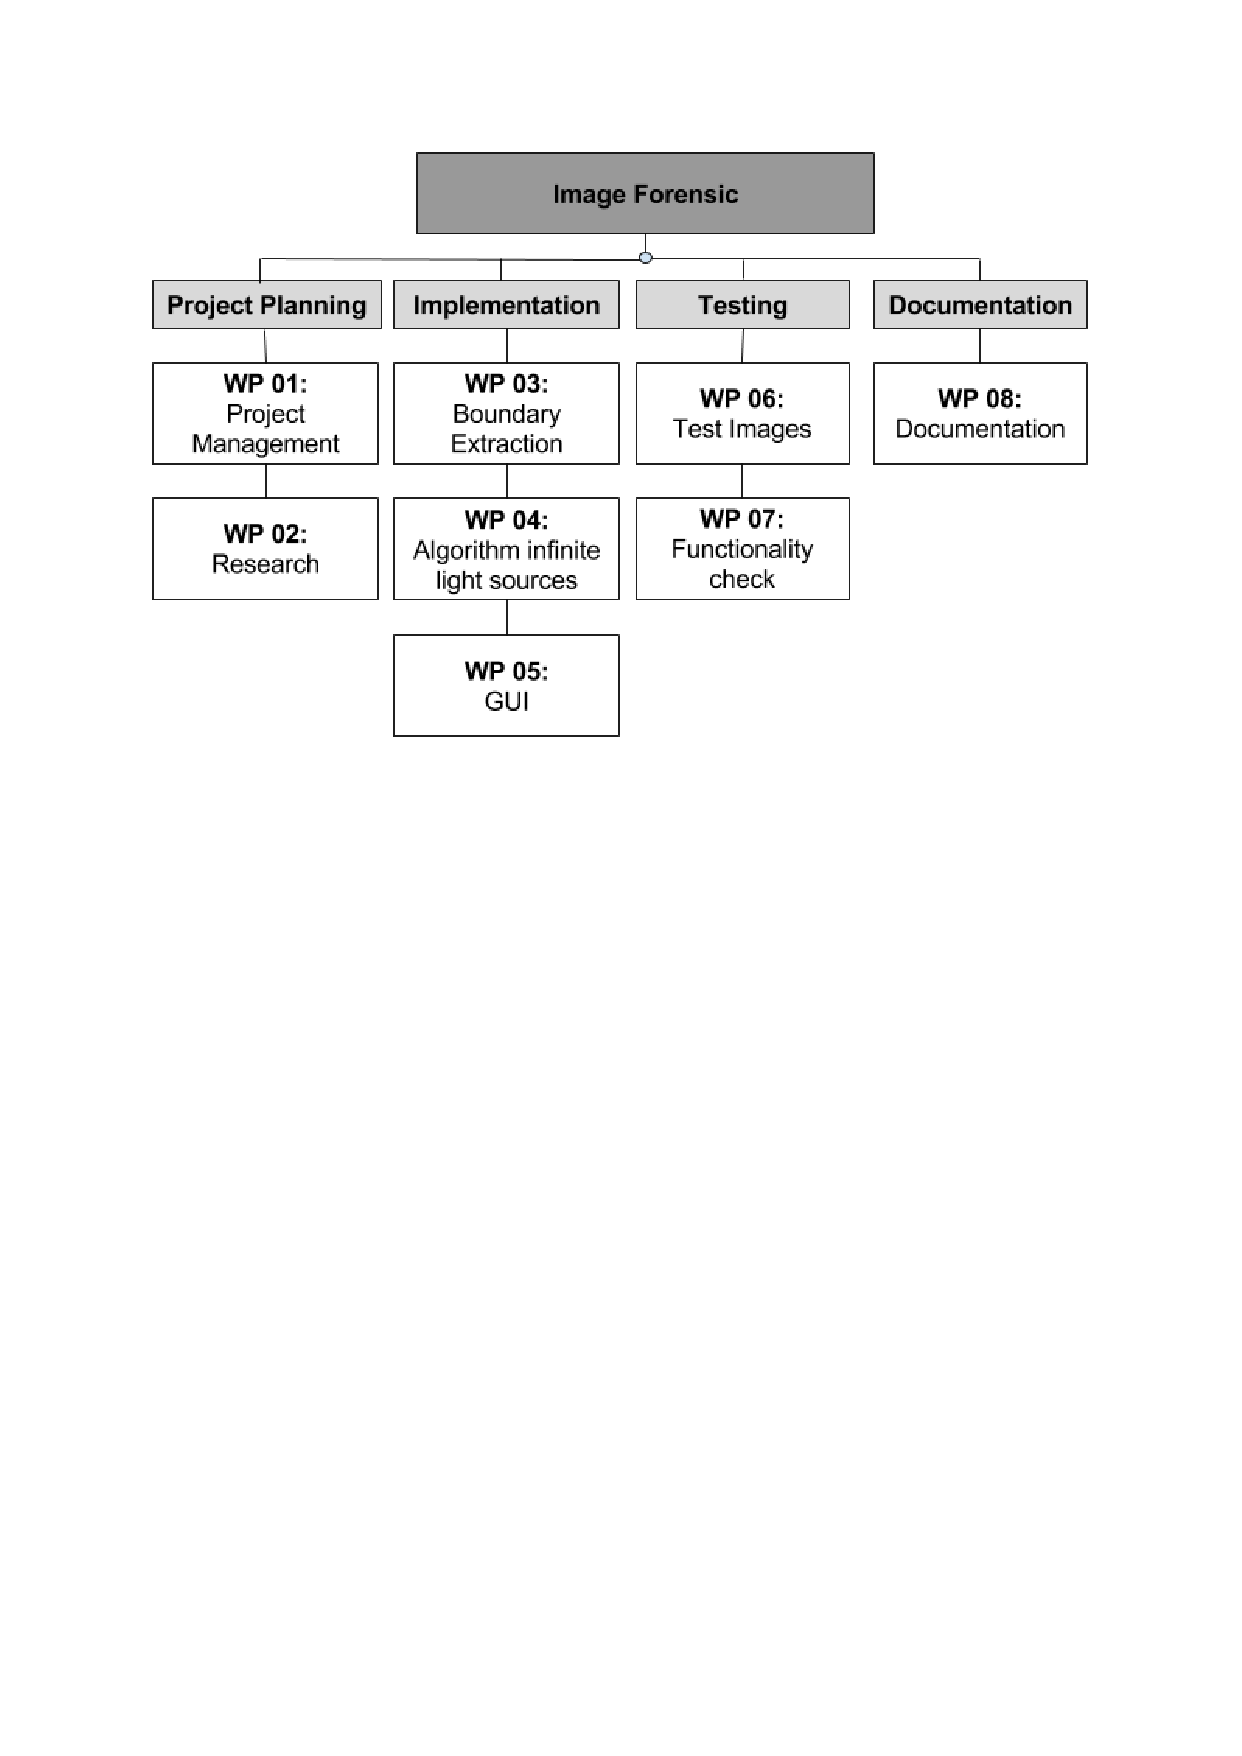
\includegraphics[scale = 0.8]{Images/Project Structure Plan.pdf}		
\end{figure}

\subsection{Milestones} \label{sec:Milestones}
\todo[inline, color=yellow]{Laura}
\begin{figure}[H] 
	\center 
	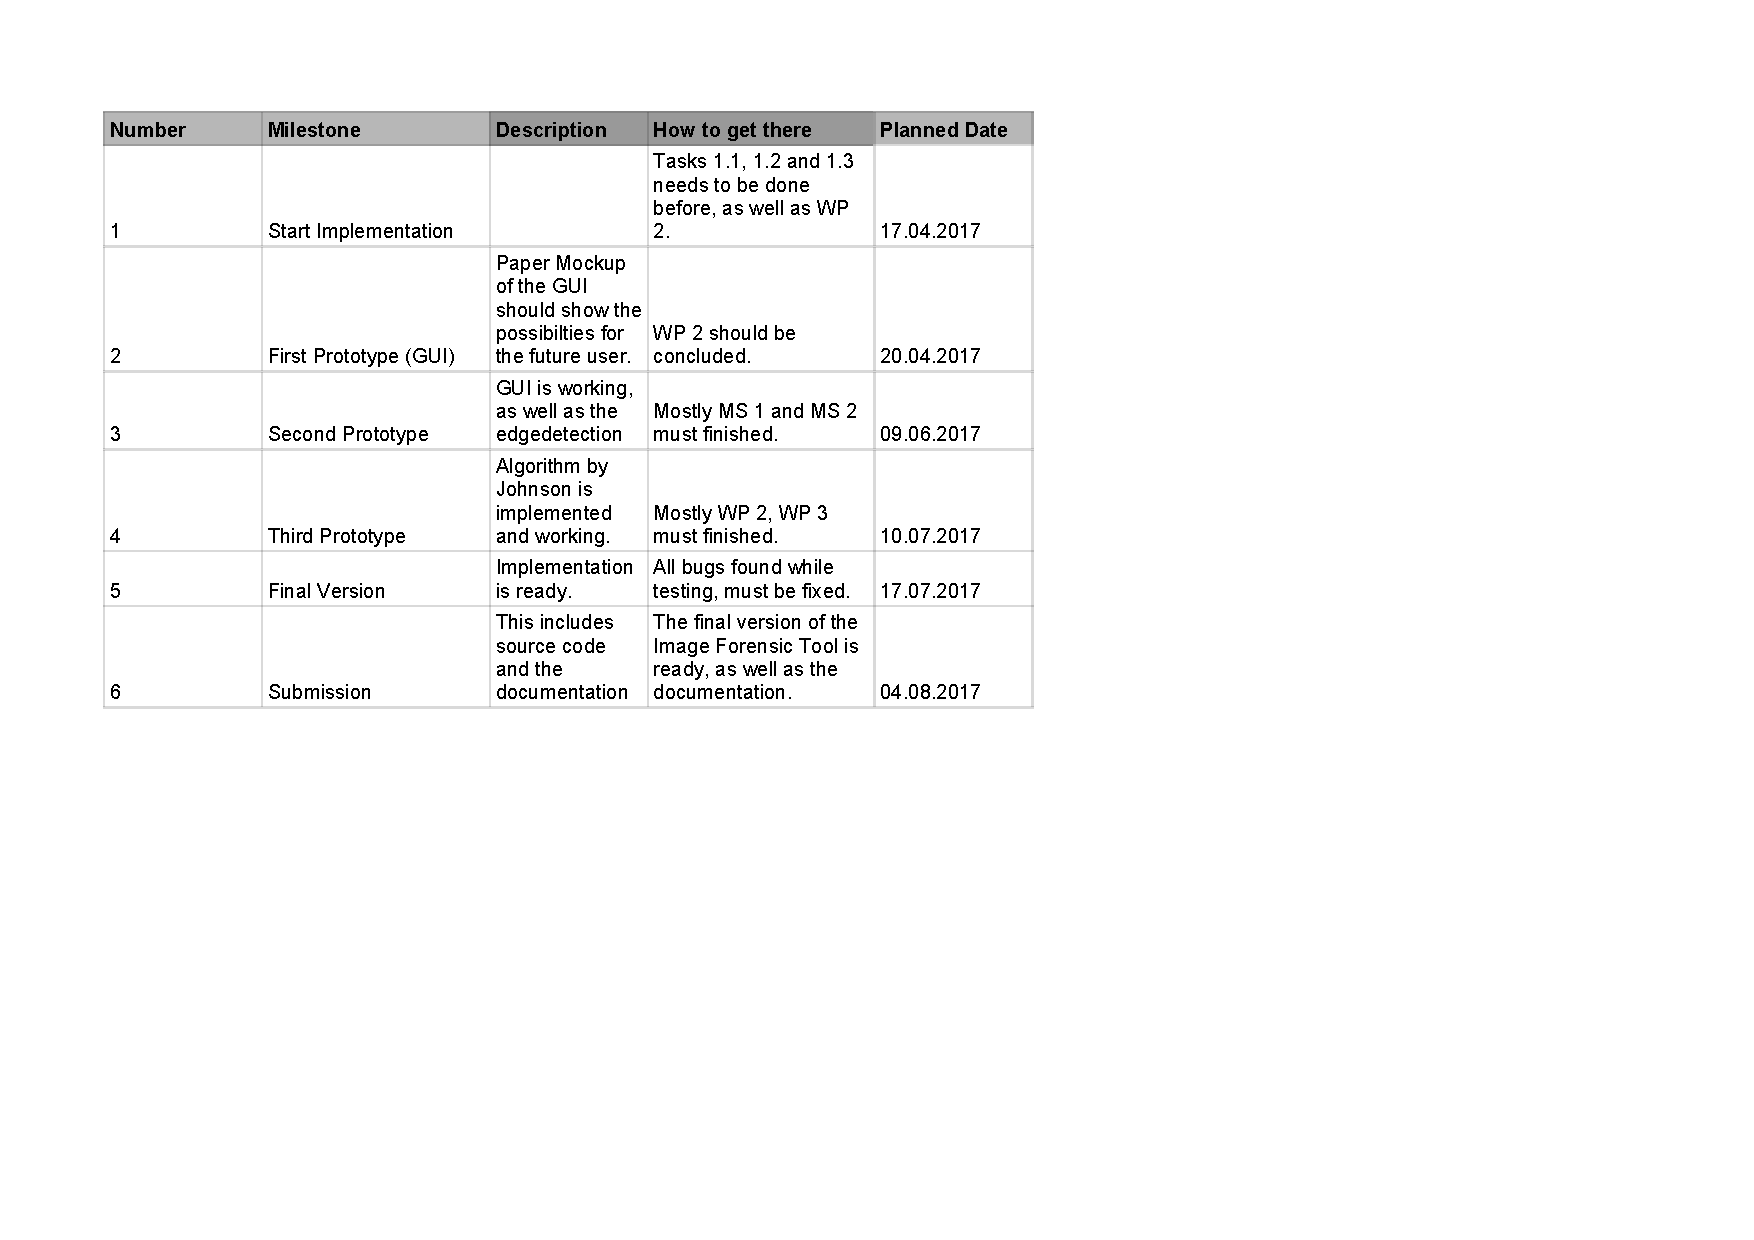
\includegraphics[scale = 0.8]{Images/milestones.pdf}		
\end{figure}

\subsection{Time Exposure} \label{sec:timeExposure}
\todo[inline, color=yellow]{Laura}
\begin{figure}[H] 
	\center 
	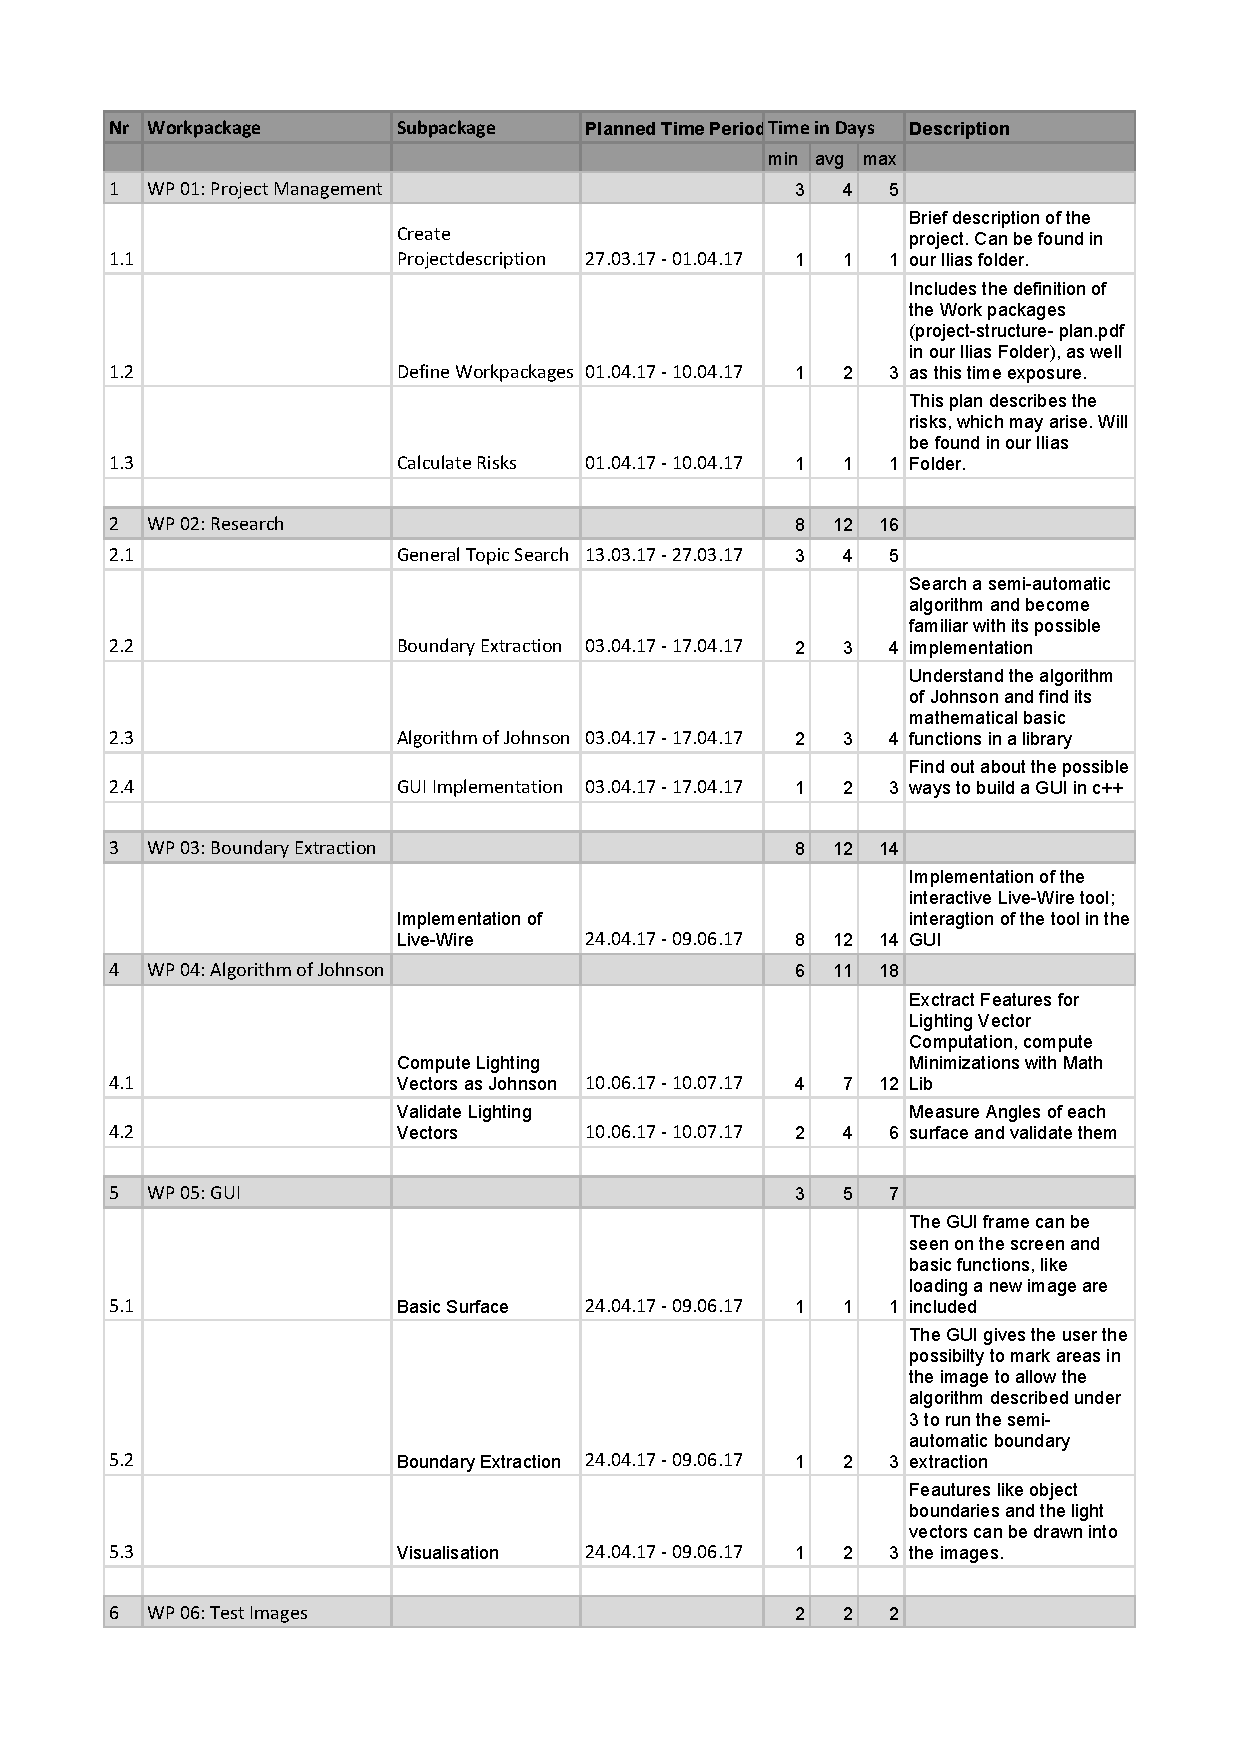
\includegraphics[scale = 0.8]{Images/Project Description and Time Exposure.pdf}		
\end{figure}



\subsection{Risks} \label{sec:risks}
\todo[inline, color=yellow]{Laura}
\begin{figure}[H] 
	\center 
	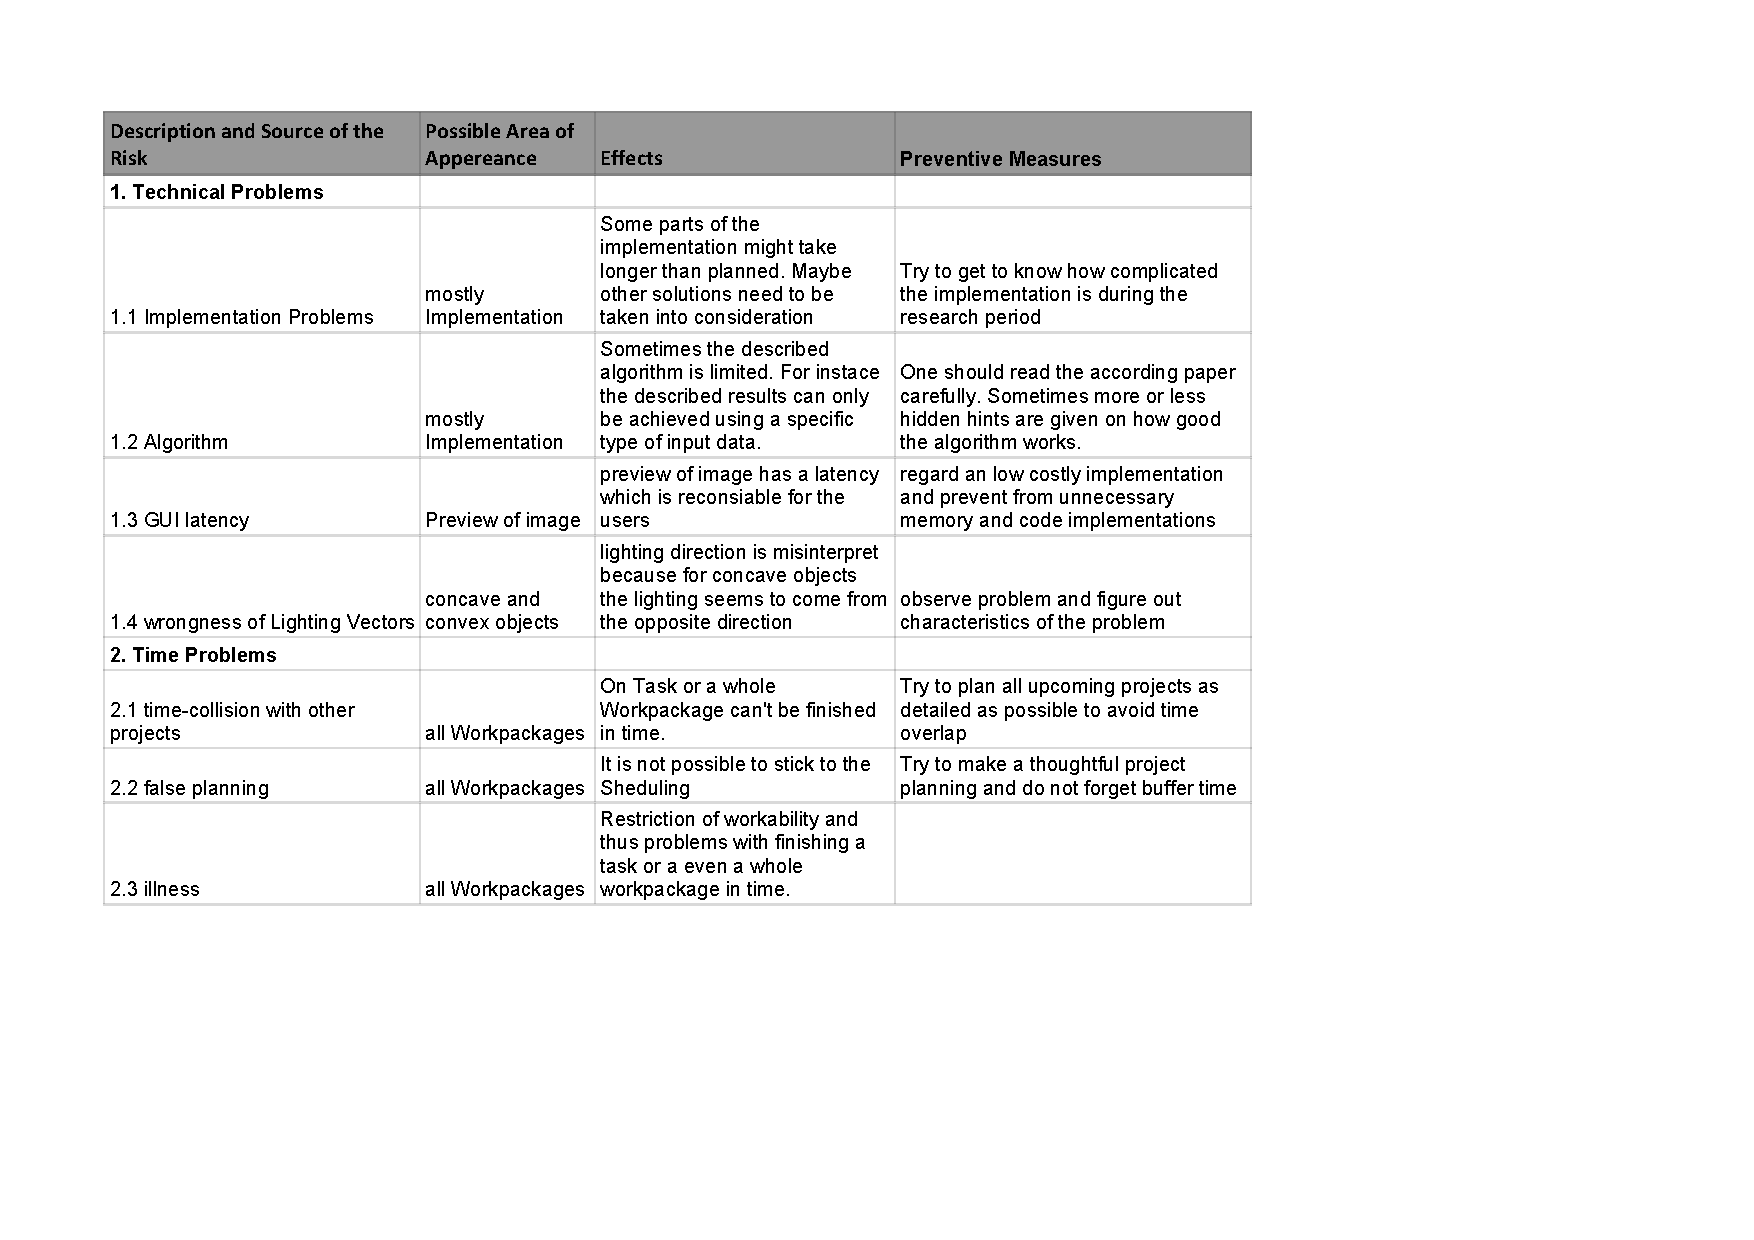
\includegraphics[scale = 0.7]{Images/risks.pdf}			
\end{figure}




\newpage


























\section{Conclusion} \label{sec:Conclusion}
\todo[inline, color=red]{Vera und Laura}

%Laura
%aufällig, dass viele ähnlich Ansätze von den Autoren selber stammen (compare section~\ref{sec:otherApproaches})
%Ansonsten Evaluation kurz zusammenfassen

\newpage































\newpage
\bibliographystyle{plain}
\bibliography{main}
\end{document}